\documentclass[12pt]{article}

 %%%%%%%%%% LOADING PACKAGES %%%%%%%%%% 
\usepackage{amsmath, amssymb, amsfonts, bm, mathtools} % math packages
\usepackage[table]{xcolor}
\usepackage{physics}
\usepackage{graphicx}
\usepackage{parskip}
\usepackage{fancyhdr}
\usepackage{vmargin}
\usepackage{tcolorbox}
\usepackage{url}
\usepackage[utf8x]{inputenc}
\usepackage{hyperref} % to click and go to pointed place in the document
\usepackage{cancel} % for easy cancellations
\usepackage{minted} % for highlighting code
\usepackage{comment} % for multi-line commenting

 %%%%%%%%%% SET DEFAULTS %%%%%%%%%% 
\newcommand{\smallspace}{\hspace{0.5cm}}
\setcounter{secnumdepth}{0} % for avoiding the numbering
\newenvironment{sfemph}{\begin{sffamily}\begin{emph}}{\end{sffamily}\end{emph}}
 % the text inside the exercise setup will be emphasized
 % Set defaults for minted
\setminted{frame=lines,
framesep=2mm,
baselinestretch=1.2,
bgcolor=,
fontsize=\footnotesize,
linenos
}

 %%%%%%%%%% INSERT YOUR DATA HERE %%%%%%%%%% 
\title{Clustering Bank Customers and
Predicting Their Loan Status}						
\author{Federico Berto}			 				
\date{\today}											
\newcommand{\professor}{Woo Chang Kim}
\newcommand{\studentid}{20204817}
\newcommand{\coursename}{Introduction to Financial Engineering}
\newcommand{\courseid}{IE471}
\newcommand{\firstuniversityline}{Korea Advanced Institute of Science} % first line of university name
\newcommand{\seconduniversityline}{and Technology} % split the title for better compatibility. You may modify this part

 %%%%%%%%%% TITLE PAGE SETUP %%%%%%%%%% 
\setmarginsrb{3 cm}{2.5 cm}{3 cm}{2.5 cm}{1 cm}{1.5 cm}{1 cm}{1.5 cm}
\makeatletter
\let\thetitle\@title
\let\theauthor\@author
\let\thedate\@date
\makeatother
\pagestyle{fancy}
\fancyhf{}
\renewcommand{\headrulewidth}{0.4pt}
\rhead{\theauthor}
\lhead{AI Project 3}
\chead{\raisebox{-1ex}{
\includegraphics[width = 3cm]{images/university_secondary_logo.png}}}
\cfoot{Page \thepage}

 %%%%%%%%%% MAIN DOCUMENT %%%%%%%%%% 
\begin{document}

 %%%%%%%%%% TITLE PAGE SETUP %%%%%%%%%% 
\begin{titlepage}
	\centering
    \textsc{\LARGE  \firstuniversityline \\ \smallskip \seconduniversityline}\\[1 cm]	% university Name
    
\includegraphics[scale = 0.18]{images/university_main_logo.png}\\[1.5 cm]	% university Logo
    
	\textsc{\Large \coursename}\\[0.5 cm]
	\rule{\linewidth}{0.2 mm} \\[0.4 cm]
	{ \huge \bfseries {\thetitle}}\\
	\rule{\linewidth}{0.2 mm} \\[1.5 cm]
	
	\begin{minipage}{0.5\textwidth}
		\begin{flushleft} \large
			\emph{Professor:}\\
		    \professor \\ [0.5cm]
            \emph{Course ID:}\\
            \courseid
			\end{flushleft}
			\end{minipage}~
			\begin{minipage}{0.4\textwidth}
			\begin{flushright} \large
			\emph{Student:} \\
			\theauthor \\[0.5cm]
			\emph{ID number:}\\
			\studentid \\
		\end{flushright}
	\end{minipage}\\[2 cm]
	
\end{titlepage}

 %%%%%%%%%% TABLE OF CONTENTS %%%%%%%%%% 
%% Uncomment this part
% \tableofcontents
% \incl
% \pagebreak


 %%%%%%%%%% MAIN TEXT %%%%%%%%%% 
\section{Introduction}


The goal of this report is to describe the experimental process and result for predicting bank loan statuses of customers based on a variety of collected data. 

In particular, we will use \textit{K-means clustering} and \textit{PCA analysis} for visualizing the clusters. As for the AI algorithms, below is a summary of each.

\subsection{AI algorithms}
\subsubsection{XGBoost}
XGBoost \cite{chen2016xgboost} is an open-source and scalable library employing regularized gradient boosting. It has become famous for winning many machine learning competitions.

\subsubsection{CatBoost}
CatBoost \cite{dorogush2018catboost} is a gradient boosting algorithm which can handle categorical values as well compared to XGBoost, by using \textit{one-hot coding}.

\subsubsection{Light GBM}
Light GBM \cite{ke2017lightgbm} improves over CatBoost's categorical feature hot-coding by using a special algorithm finding the split value of categorical features, Gradient-based One-Side Sampling (GOSS).

\subsubsection{Multilayer Perceptron Classification with Imbalanced Datasets}
Multilayer Perceptrons with Imbalanced Datasets \cite{he2009learning} are very different in terms of structure compared to the previous algorithms. We use Deep Learning and Backpropagation for obtaining the optimal weights minimizing a loss function. Moreover, weighting and other techniques improve over the dataset imbalance. 

\subsection{Explainable AI}
In order to provide a better visualization to the results, we use Explainable AI (XAI). In particular we will employ these two algorithms:
\begin{enumerate}
    \item \textbf{LIME}: Local Interpretable Model-Agnostic Explanations \cite{DBLP:journals/corr/RibeiroSG16} , this learns a locally interpretable prediction model for any classifier.
    \item \textbf{SHAP}: SHapley Additive exPlanations \cite{DBLP:journals/corr/LundbergL17}, this algorithm used class importance features for showing human-understandable machine learning.
\end{enumerate}



\section{Experiments}

\subsection{Clustering and prediction for Kaggle's Bank Loan Status Dataset}
In this section we provide the required data for the report based on the Kaggle's Bank Loan Status Dataset \footnote{Source: \href{https://www.kaggle.com/zaurbegiev/my-dataset}{Kaggle}}.

\paragraph{1.} K-means cluster plot with the PCA results (Figure \ref{fig:pca_kaggle})

\begin{figure}[h!]
    \centering
    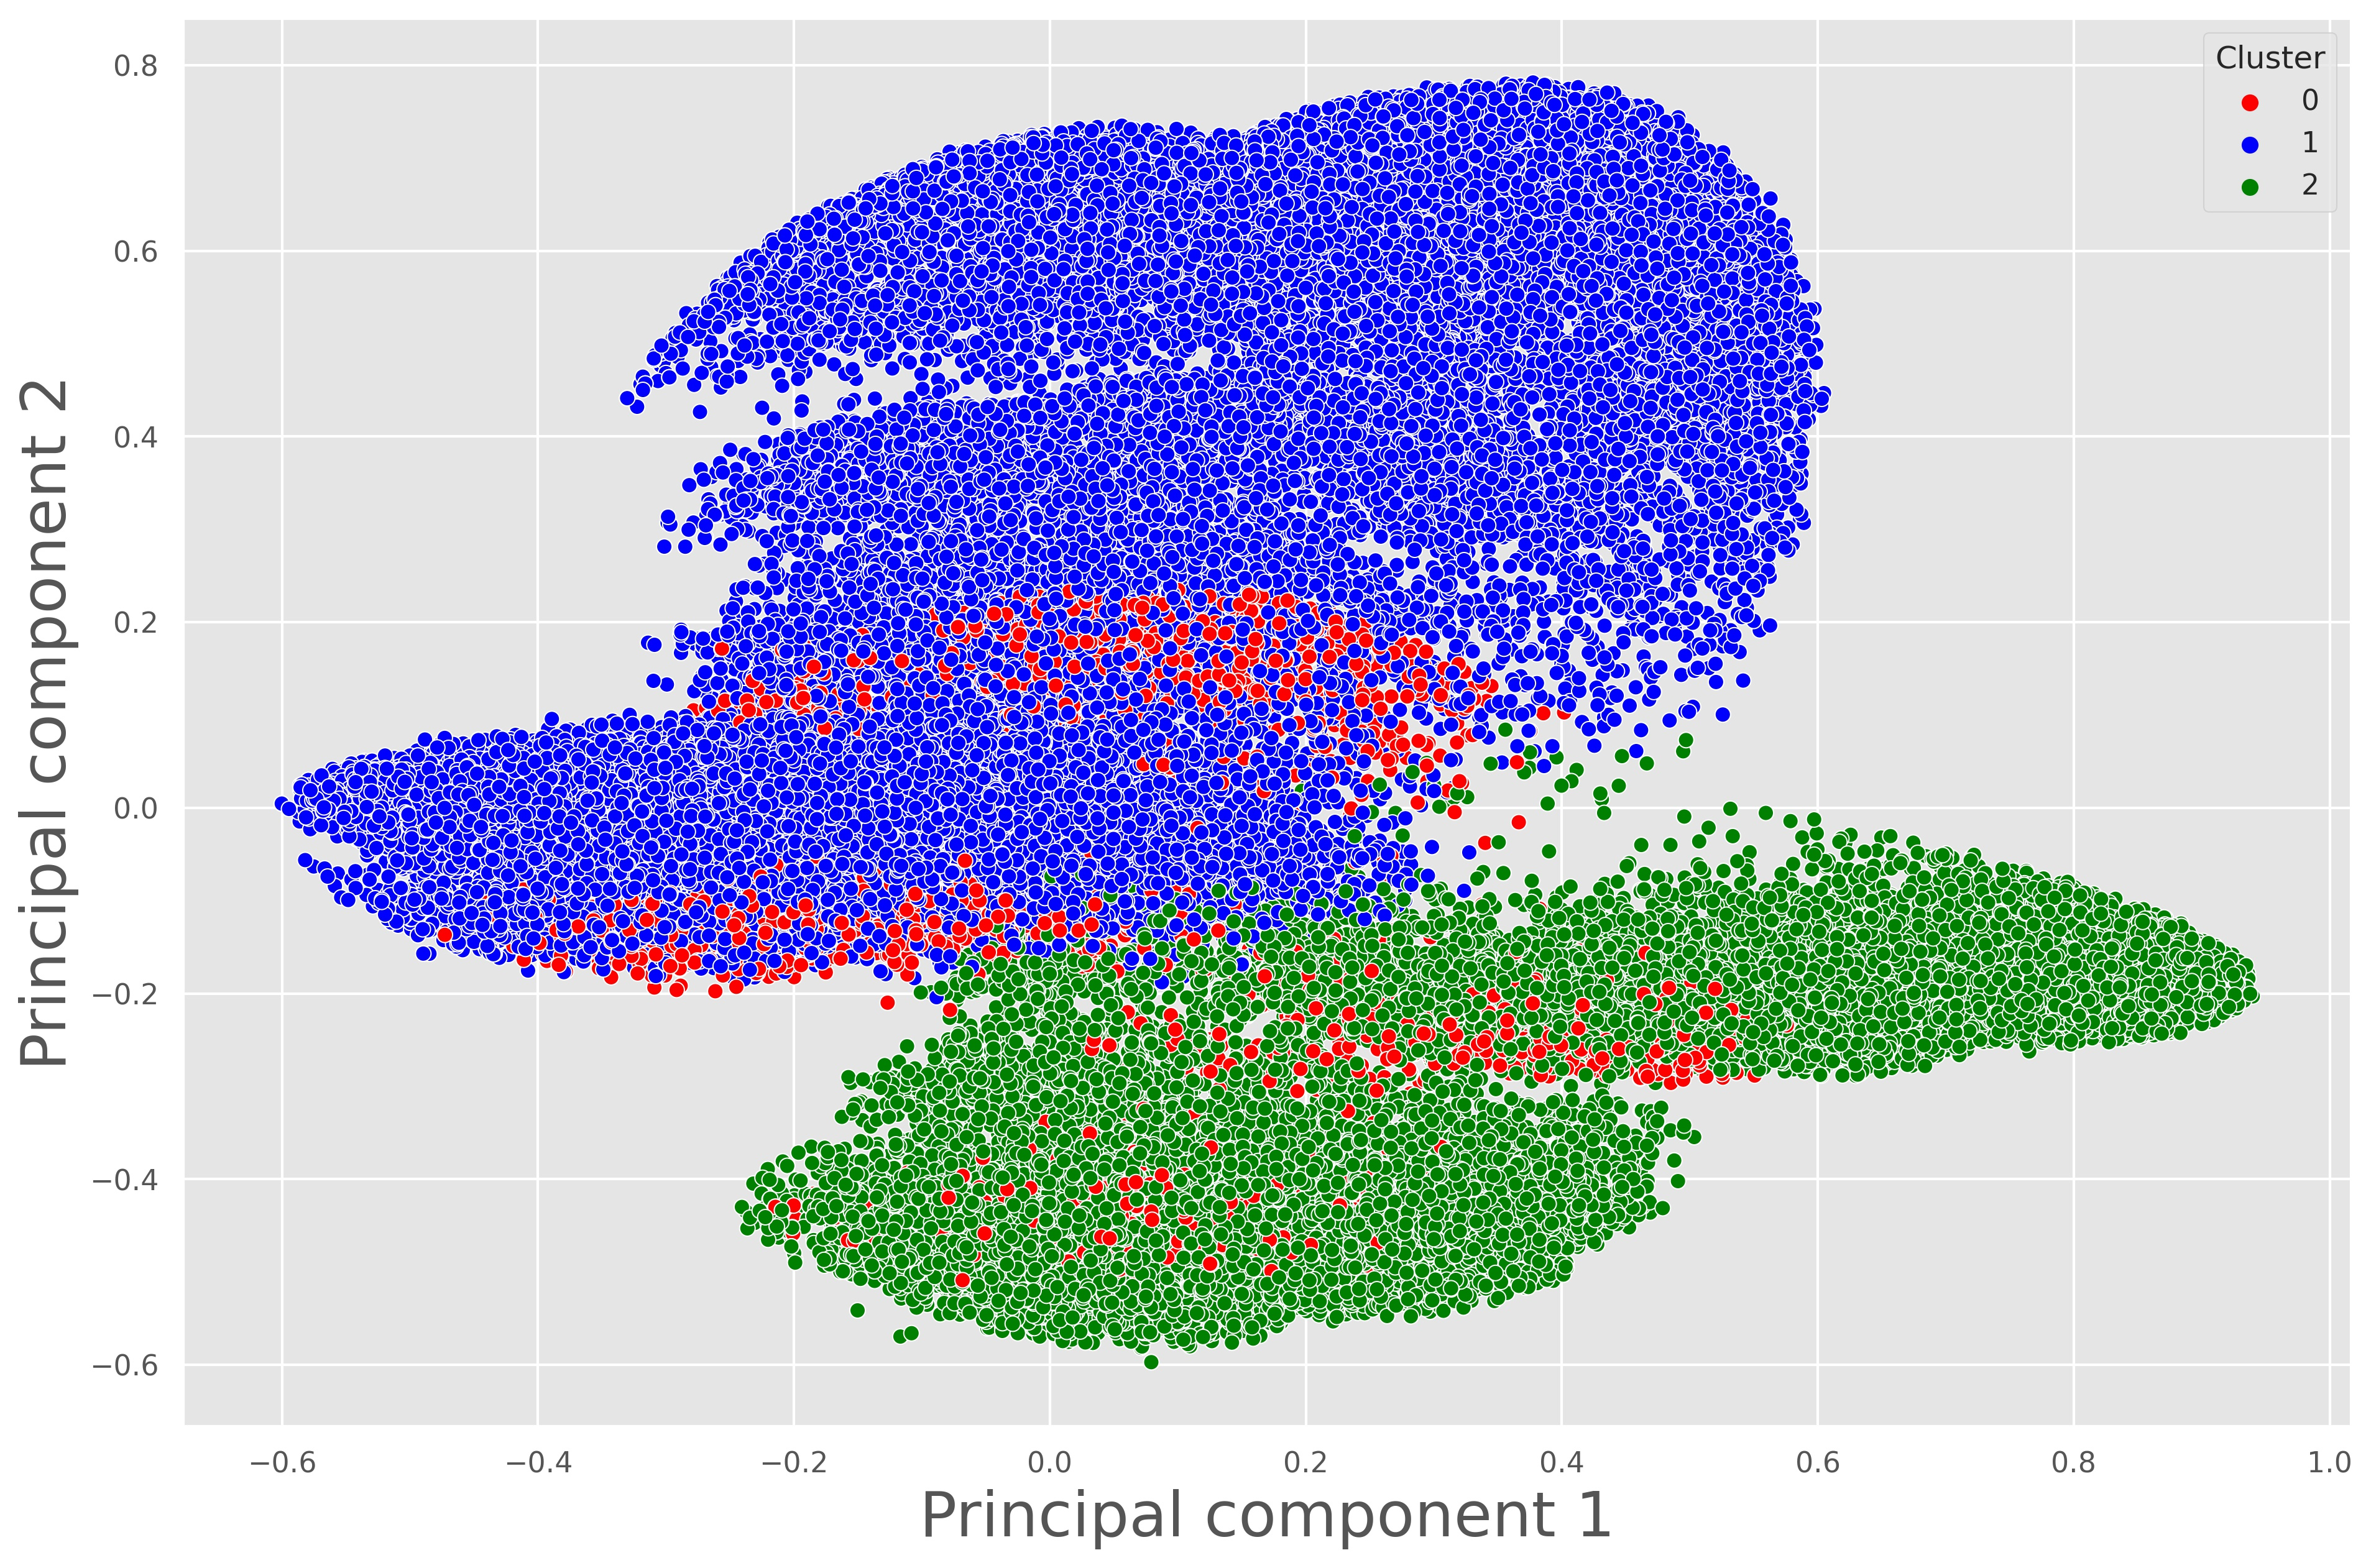
\includegraphics[width=0.9\textwidth]{images/pca_results_kaggle.jpg}
    \caption{PCA results on the clustering}
    \label{fig:pca_kaggle}
\end{figure}


\paragraph{2.} Comparison of the loan status proportion of those three clusters:
\begin{center}
\rowcolors{2}{gray!25}{white}     
    \begin{tabular}{l l l l l}
    \rowcolor{gray!50}
         \textbf{Loan Status} & \textbf{Mean} & \textbf{Cluster 0} & \textbf{Cluster 1} & \textbf{Cluster 2}\\
         \hline
         \text{Charged Off} & 22.6336 & 19.952 & 19.9007  &30.3494\\
         \text{Fully Paid} & 77.3664 & 80.048 & 80.0993 & 69.6506 \\
    \end{tabular}
\end{center}

As we can see from this analysis, the K-means algorithm grouped the customers in three main clusters: while the first two (Clusters 0 and 1) have roughly an 80-20 ratio of people who managed to pay the loan and people who were charged off, Cluster 2 has a much higher ratio of people who could not pay off the loan (more than $30\%$). Therefore, it is more probable for people in this cluster to \textit{default} the payment and be untrustworthy to the bank.

\paragraph{3.} Columns, non-null count in those columns, and data type of original data using $\tt credit.info()$:
\begin{center}
\rowcolors{2}{gray!25}{white}     
    \begin{tabular}{l l l l}
    \rowcolor{gray!50}
	\textbf{Feature No.} & \textbf{Value} & \textbf{Number} & \textbf{Type} \\	% of Total Values
 0  & Loan ID                  &     100000 non-null &  object \\
 1   &Customer ID               &    100000 non-null & object \\
 2  & Loan Status               &    100000 non-null & object  \\
 3  & Current Loan Amount       &    100000 non-null & float64 \\
 4  & Term                      &    100000 non-null & object \\
 5  & Credit Score              &    80846 non-null  & float64\\
 6  & Annual Income             &    80846 non-null  & float64\\
 7  & Years in current job      &    95778 non-null  & object \\
 8  & Home Ownership            &    100000 non-null & object \\
 9  & Purpose                   &    100000 non-null & object \\
 10 & Monthly Debt              &    100000 non-null & float64\\
 11 & Years of Credit History   &    100000 non-null & float64\\
 12 & Months since last delinquent & 46859 non-null  & float64\\
 13 & Number of Open Accounts   &    100000 non-null & float64\\
 14 & Number of Credit Problems  &   100000 non-null & float64\\
 15 & Current Credit Balance     &   100000 non-null & float64\\
 16 & Maximum Open Credit        &   99998 non-null  & float64\\
 17 & Bankruptcies               &   99796 non-null  & float64\\
 18 & Tax Liens                  &   99990 non-null  & float64\\
    \end{tabular}
\end{center}

\paragraph{4.} Count plot of the \textit{Years in current job} feature:

\begin{figure}[h!]
    \centering
    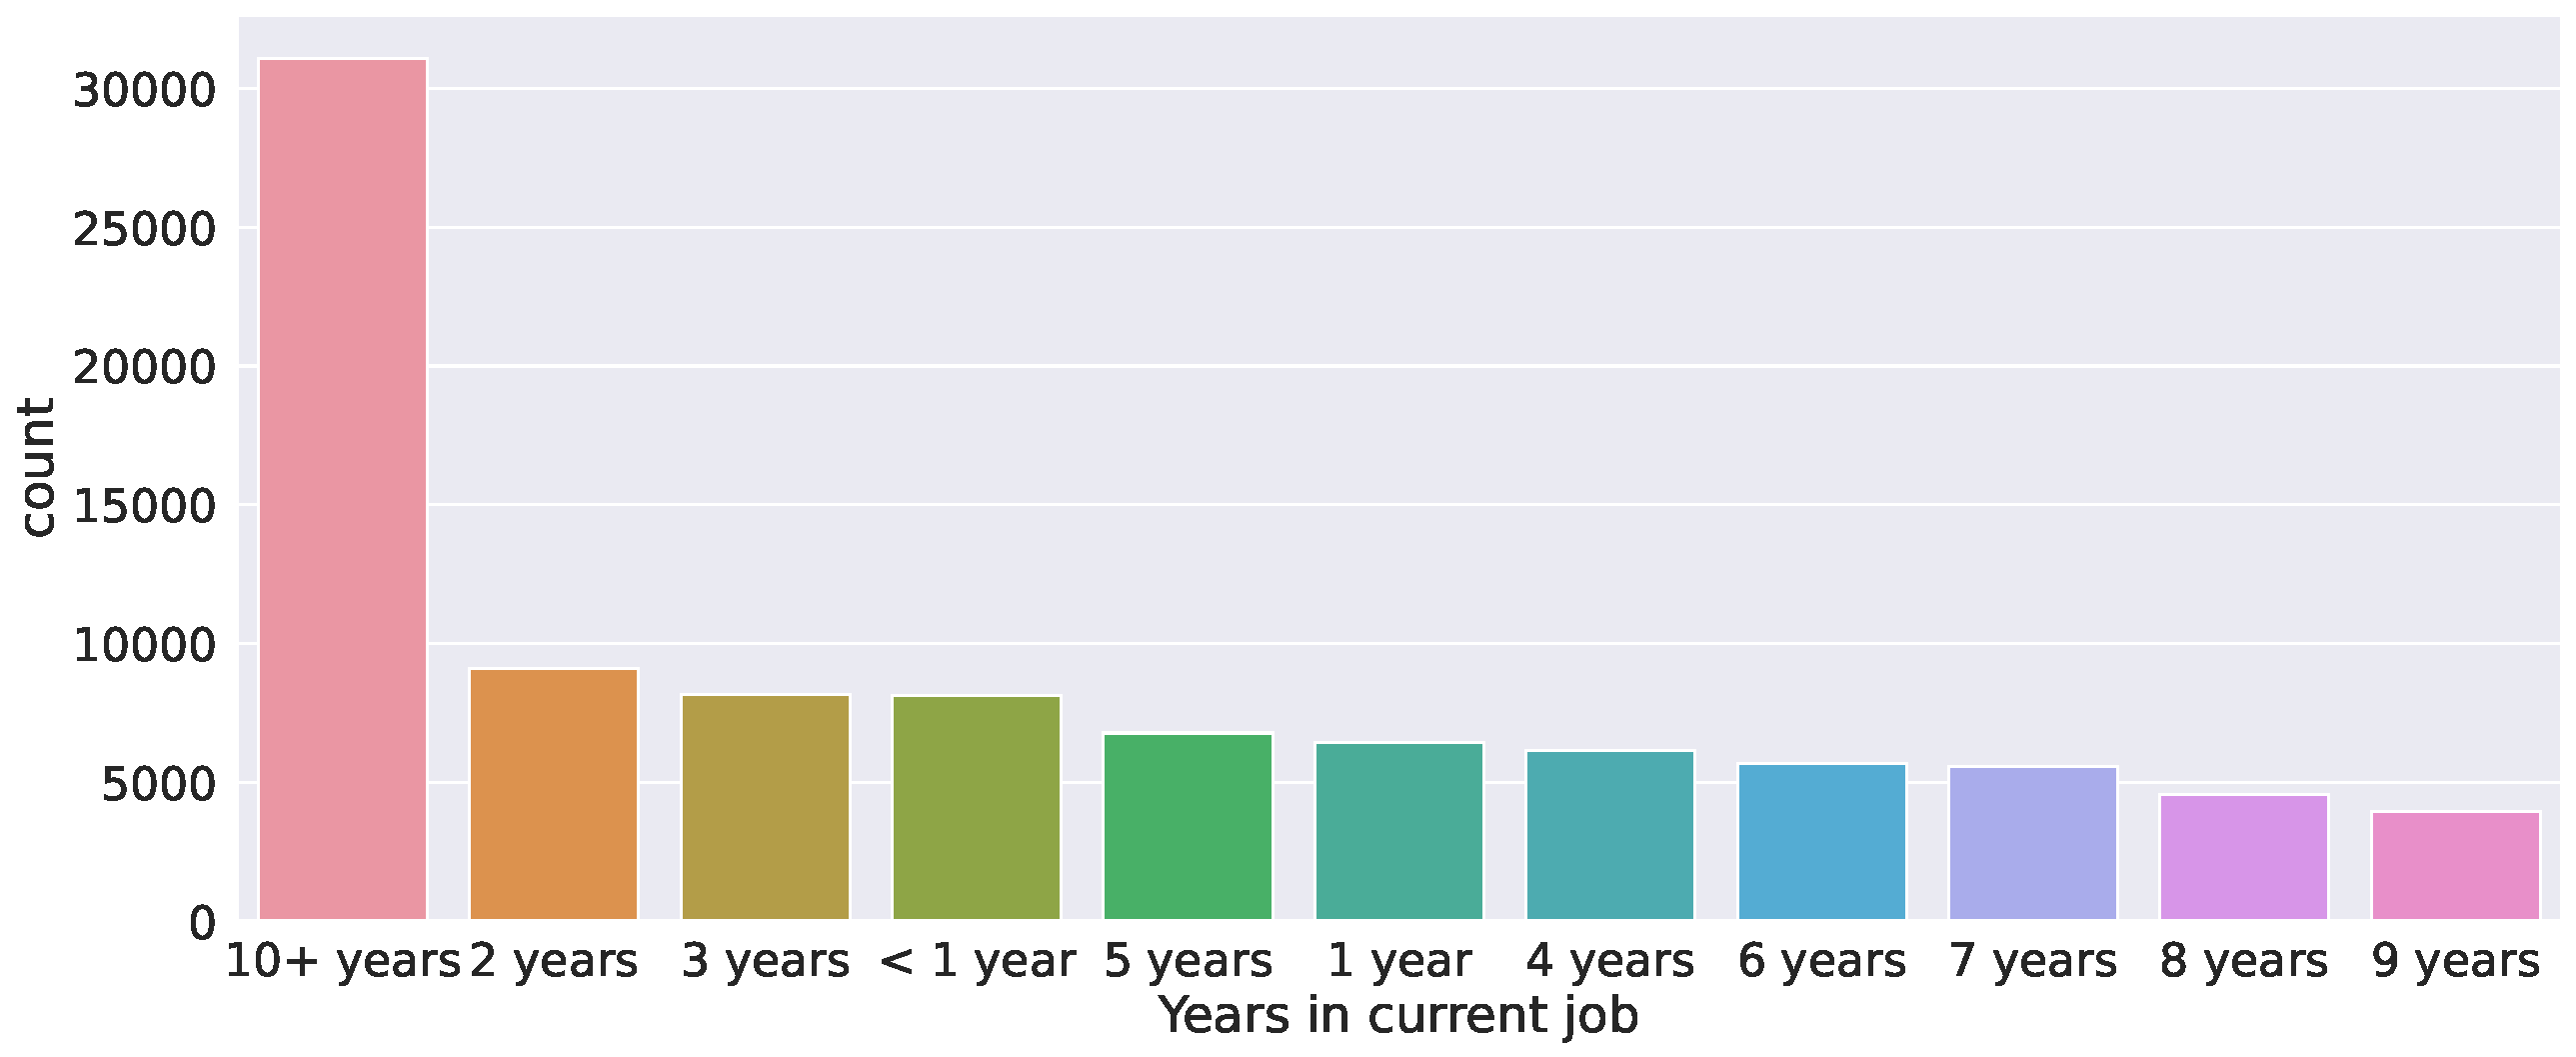
\includegraphics[width=0.9\textwidth]{images/countplot.pdf}
    \caption{Count plot of years in the current job}
    \label{fig:countplot_kaggle}
\end{figure}

\paragraph{5.} Shapley value of 14th datum is $1.97$ and the analysis result is as following:
\begin{figure}[h!]
    \centering
    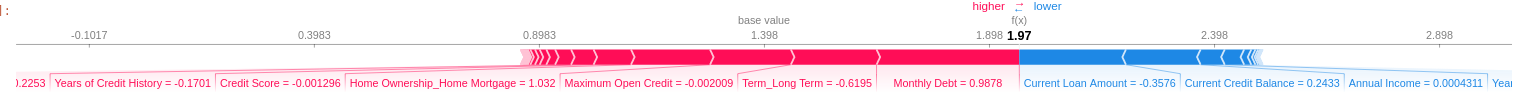
\includegraphics[width=1.\textwidth]{images/forceplot.png}
    \caption{Force plot of the 14th datum}
    \label{fig:forceplot_kaggle}
\end{figure}


\paragraph{6.} Summary of all feature effects and description:
\begin{figure}[h!]
    \centering
    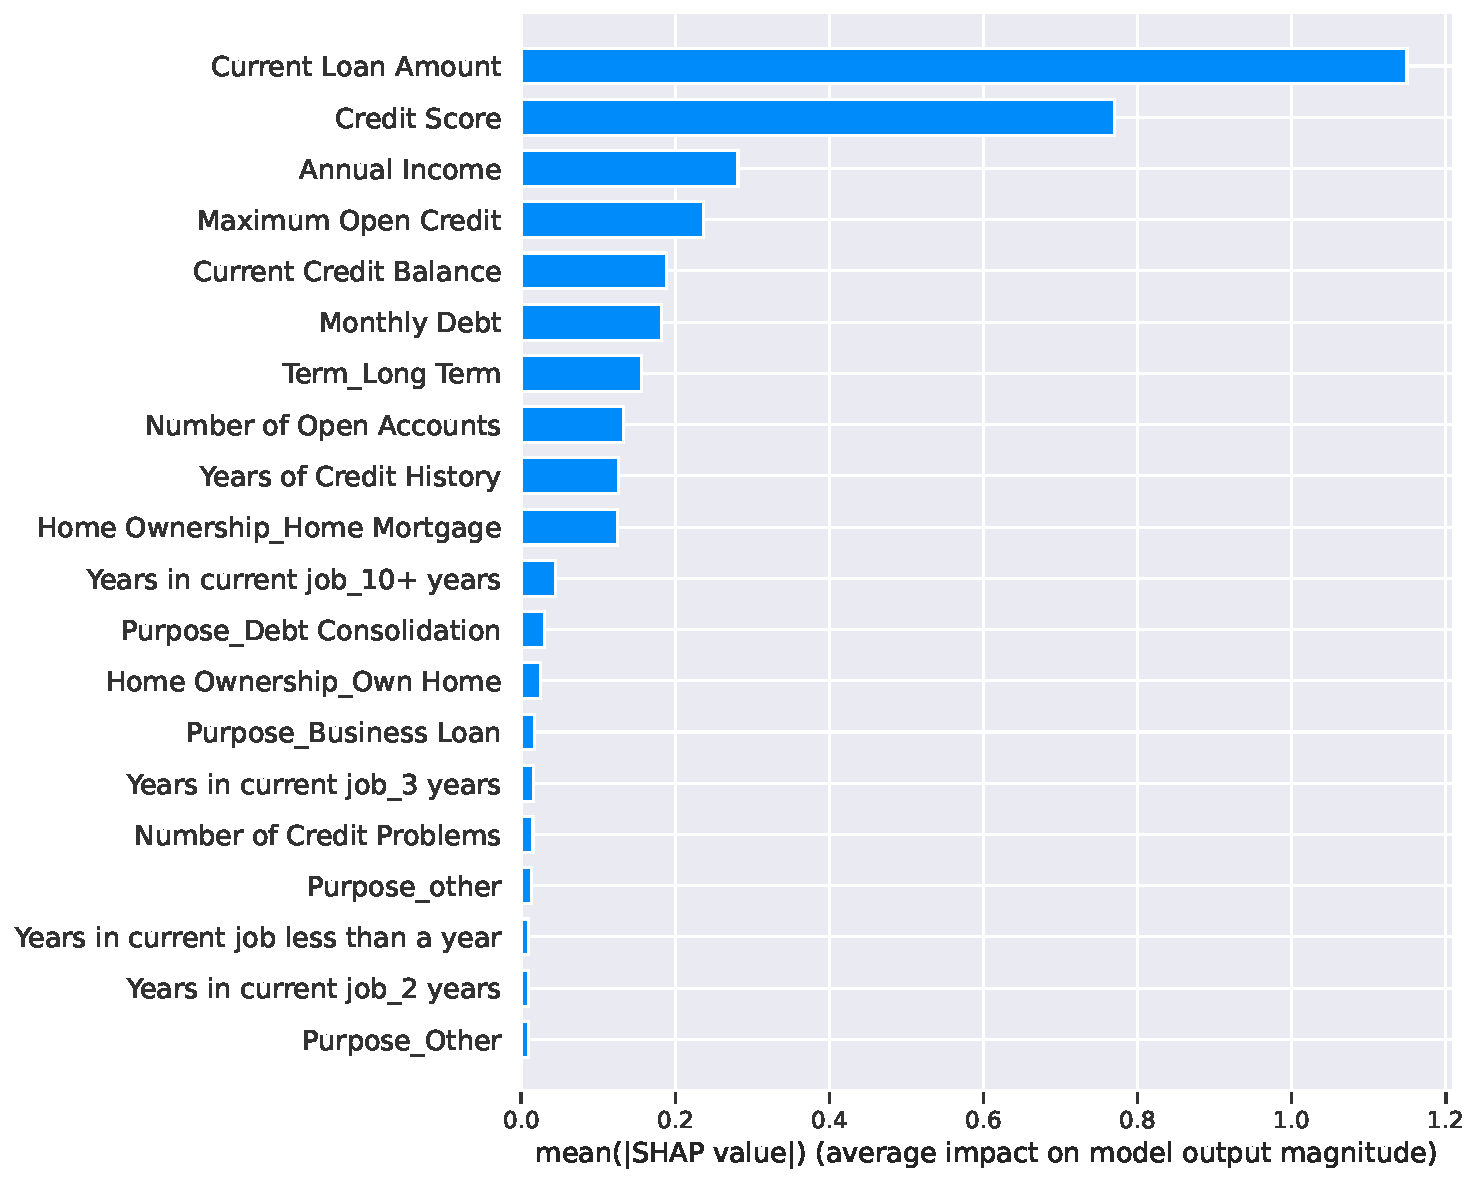
\includegraphics[width=0.9\textwidth]{images/summary_plot_bar_kaggle.pdf}
    \caption{Bar summary plot with SHAP}
    \label{fig:barplot_kaggle}
\end{figure}

\begin{figure}[h!]
    \centering
    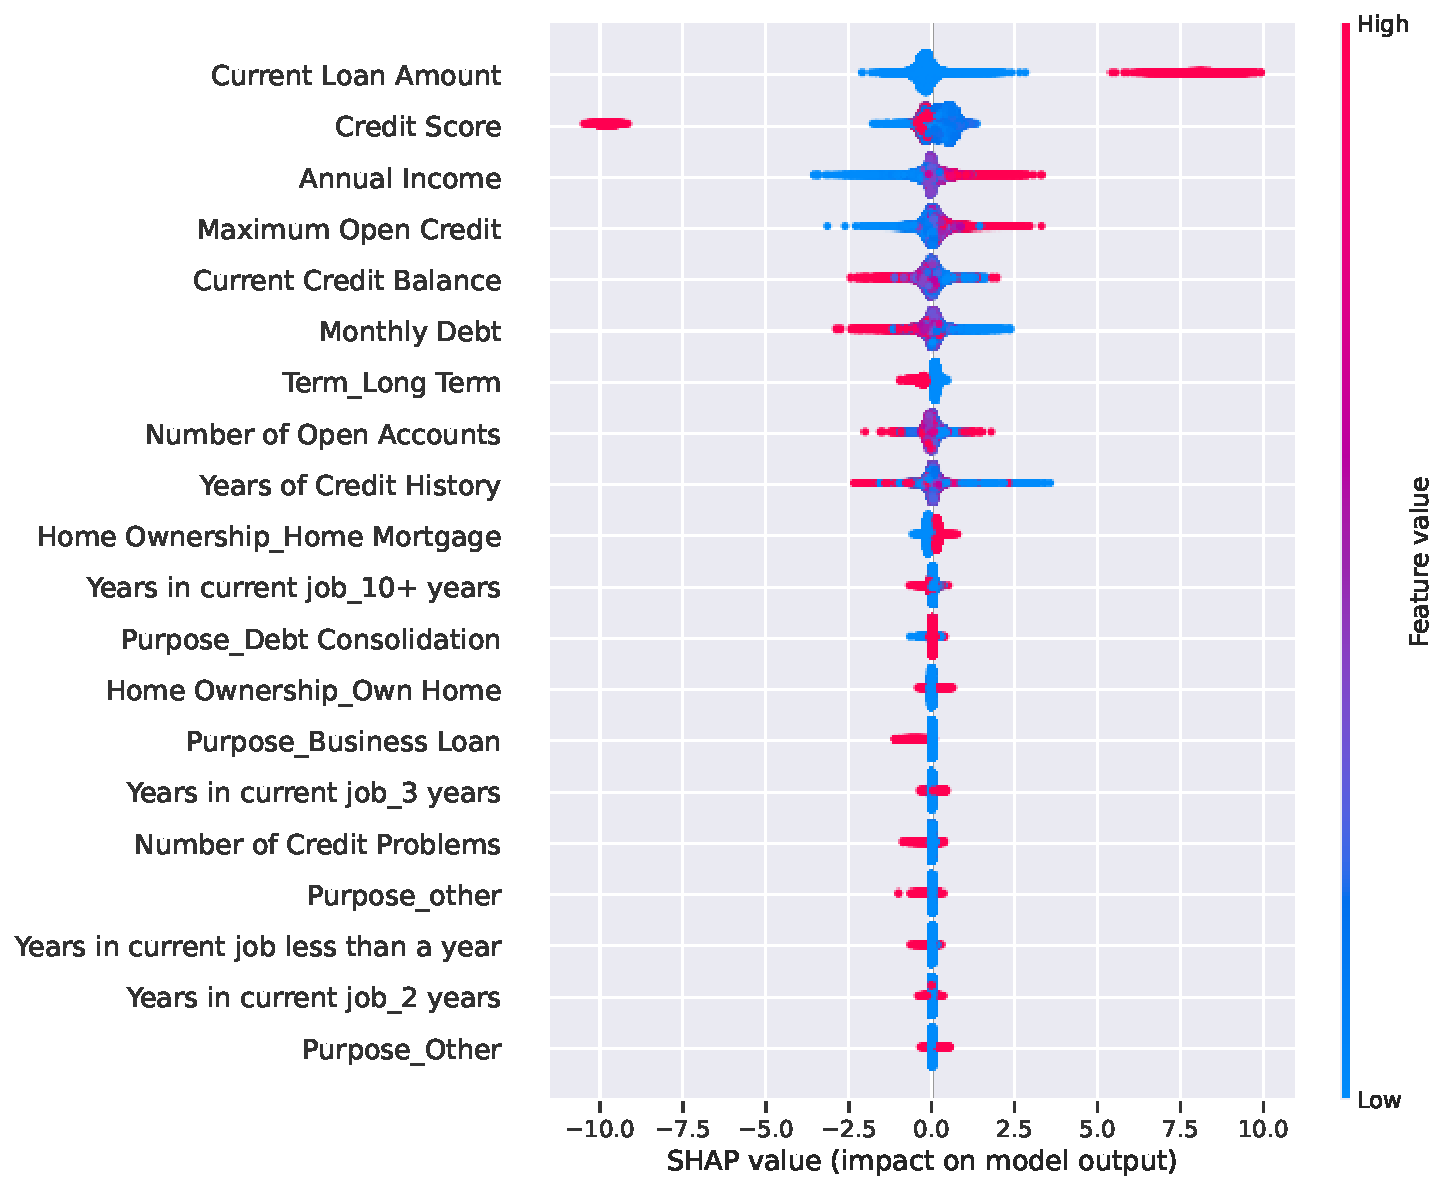
\includegraphics[width=0.9\textwidth]{images/summary_plot_kaggle.pdf}
    \caption{Tree summary plot with SHAP}
    \label{fig:treesum_kaggle}
\end{figure}


\begin{figure}[h!]
    \centering
    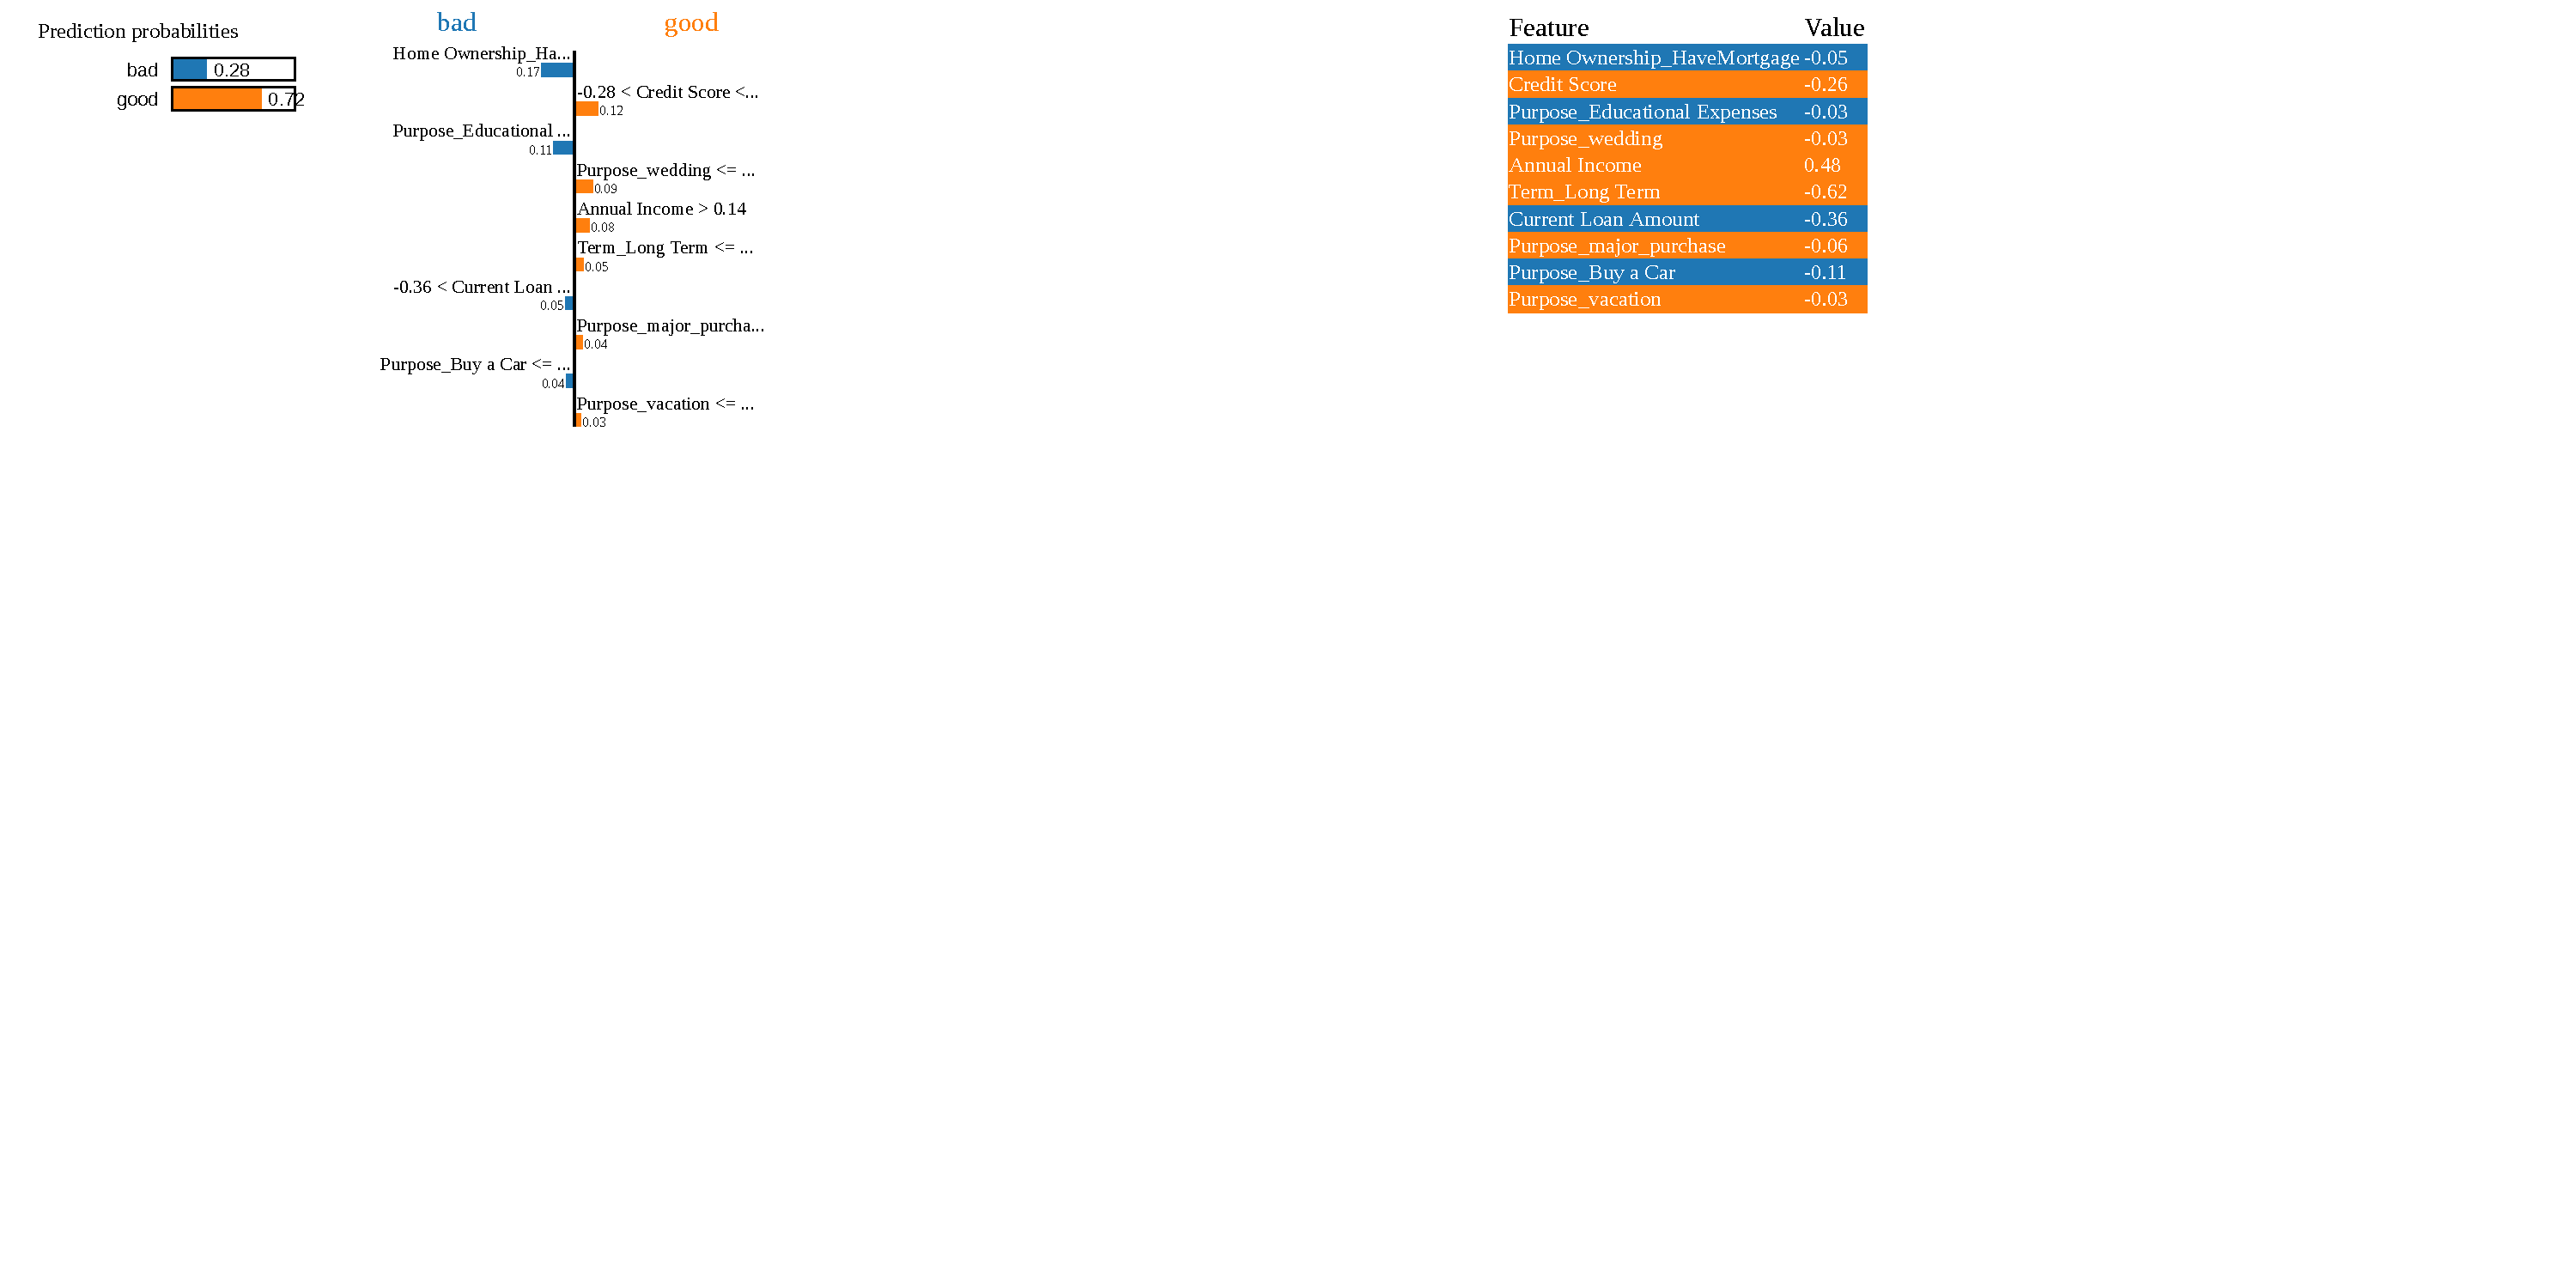
\includegraphics[width=1.\textwidth]{images/lime.pdf}
    \caption{Summary with LIME showing "good" and "bad" feature depending on our prediction labels}
    \label{fig:lime_kaggle}
\end{figure}

Figures \ref{fig:forceplot_kaggle} and \ref{fig:barplot_kaggle} show the importance of the features based on the SHAP values, while Figure \ref{fig:lime_kaggle} shows the features importance based on LIME, another Explainable AI algorithm. 

As we can see from the analysis, the most import three features are the Current Loan Amount, Credit Score and the Annual Income. In particular, the SHAP values show that high values of Current Loan Amount and Annual Income are positively correlated to the prediction, while high values of credit score are negatively correlated to it.

\section{Analyzing and improving the Predictions}
\subsection{AI algorithms}
In this section, we will analyze the prediction results on the test dataset by comparing $\tt XGBoost$ to other boosting algorithms: $\tt CatBoost$ and $\tt LightGBM$.

Moreover, we also implement a version of Multilayer Perceptrons with Pytorch Lightning \cite{falcon2019pytorch} and and \textit{Imbalanced Dataset Sampler} to compare the results of Deep Learning and Boosting Algorithms.

In order to compare the results, we will use \textit{confusion matrices}, which are a simple way of visualizing classification results. Moreover, we will not only employ Mean Squared Error, but also \textit{precision} and \textit{recall} measures to have a better understanding of how the algorithms perform.

\subsection{Results}

\begin{figure}
\centering
    \begin{minipage}{0.45\textwidth}
      \centering
      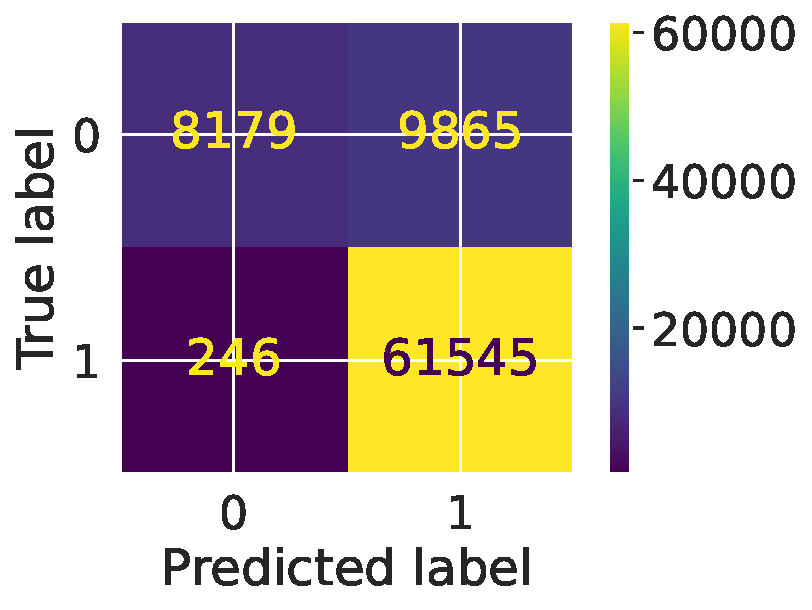
\includegraphics[width=.9\linewidth]{images/xboost_confusion_matrix_train.pdf}
      \caption{Train dataset confusion matrix for XGBoost}
      \label{fig:cm_xgboost_train}
    \end{minipage} \hfill
    \begin{minipage}{0.45\textwidth}
      \centering
      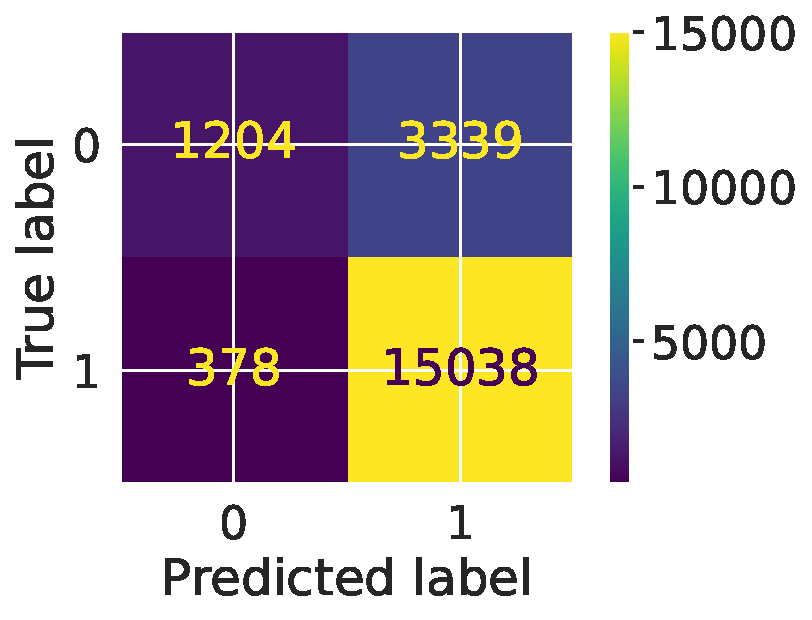
\includegraphics[width=.9\linewidth]{images/xboost_confusion_matrix_test.pdf}
      \caption{Test dataset confusion matrix for XGBoost}
      \label{fig:cm_xgboost_test}
    \end{minipage}
\end{figure}

\begin{figure}
\centering
    \begin{minipage}{0.45\textwidth}
      \centering
      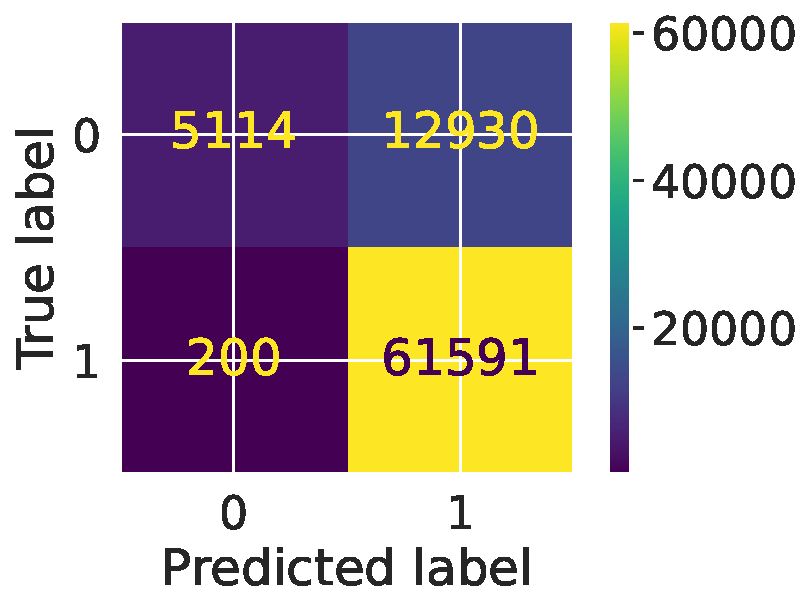
\includegraphics[width=.9\linewidth]{images/catboost_confusion_matrix_train.pdf}
      \caption{Train dataset confusion matrix for CatBoost}
      \label{fig:cm_catboost_train}
    \end{minipage} \hfill
    \begin{minipage}{0.45\textwidth}
      \centering
      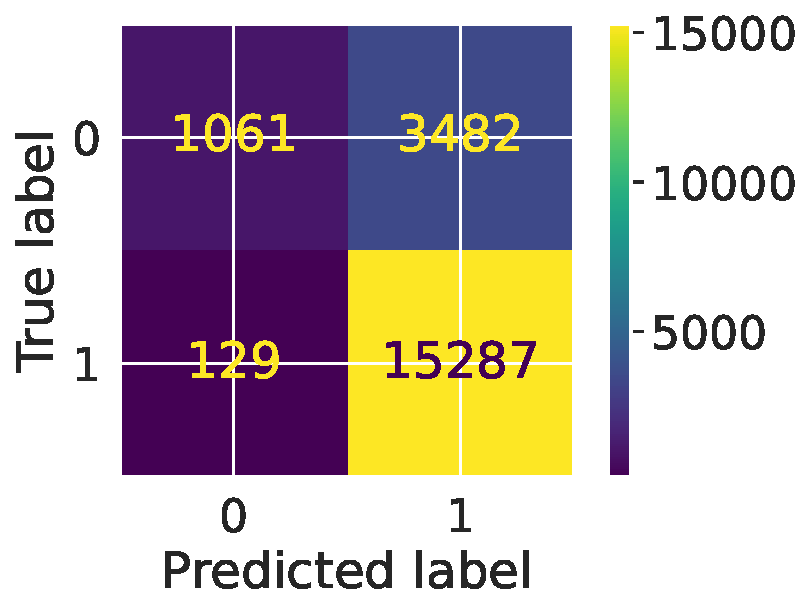
\includegraphics[width=.9\linewidth]{images/catboost_confusion_matrix_test.pdf}
      \caption{Test dataset confusion matrix for CatBoost}
      \label{fig:cm_catboost_test}
    \end{minipage}
\end{figure}

\begin{figure}
\centering
    \begin{minipage}{0.45\textwidth}
      \centering
      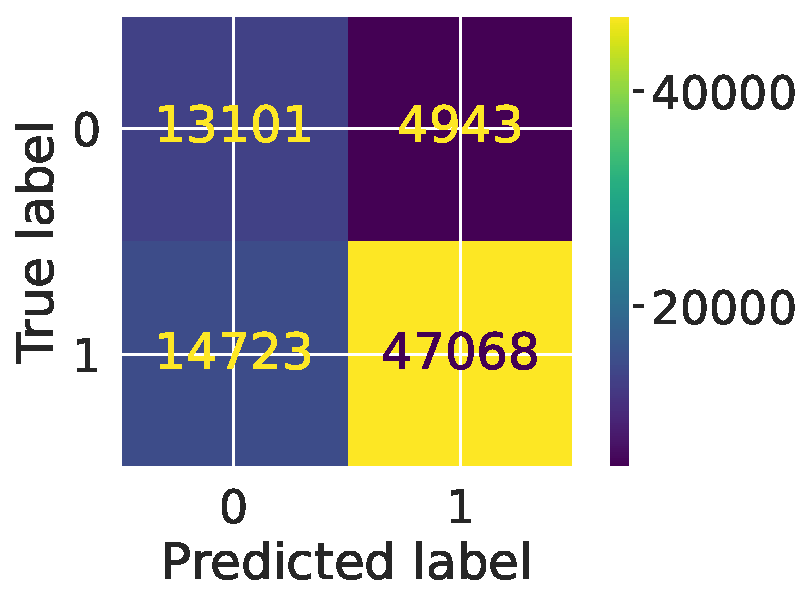
\includegraphics[width=.9\linewidth]{images/lightgbm_confusion_matrix_train.pdf}
      \caption{Train dataset confusion matrix for Light GBM}
      \label{fig:cm_lightgbm_train}
    \end{minipage} \hfill
    \begin{minipage}{0.45\textwidth}
      \centering
      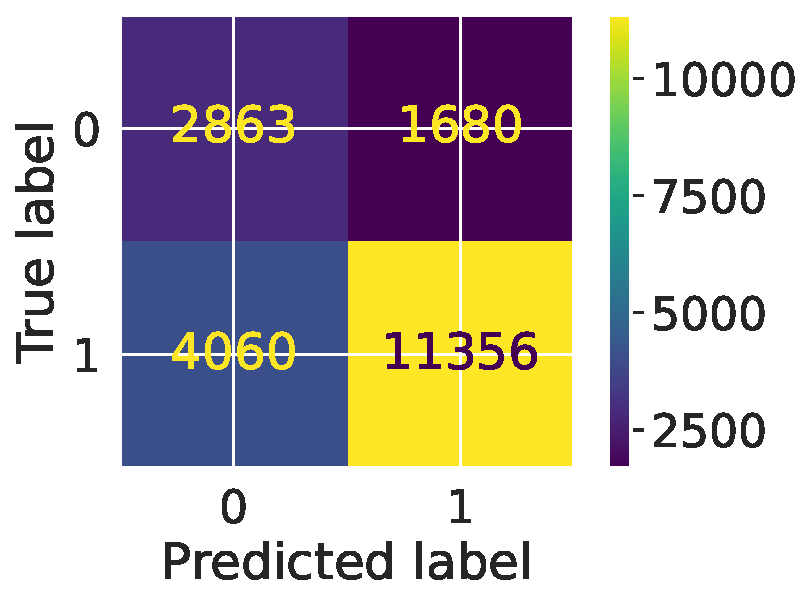
\includegraphics[width=.9\linewidth]{images/lightgbm_confusion_matrix_test.pdf}
      \caption{Test dataset confusion matrix for Light GBM}
      \label{fig:cm_lightgbm_test}
    \end{minipage}
\end{figure}

\begin{figure}
\centering
    \begin{minipage}{0.45\textwidth}
      \centering
      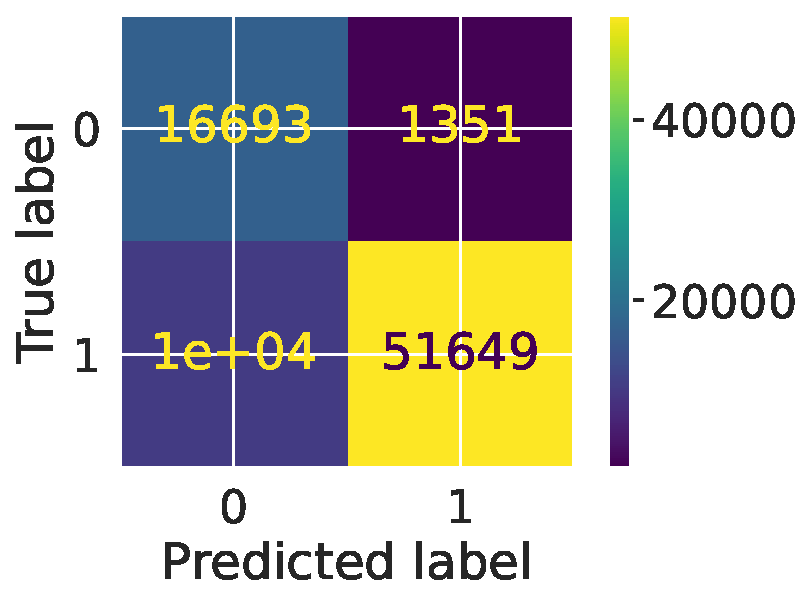
\includegraphics[width=.9\linewidth]{images/mlp_confusion_matrix_train.pdf}
      \caption{Train dataset confusion matrix for the Multilayer Perceptron}
      \label{fig:cm_mlp_train}
    \end{minipage} \hfill
    \begin{minipage}{0.45\textwidth}
      \centering
      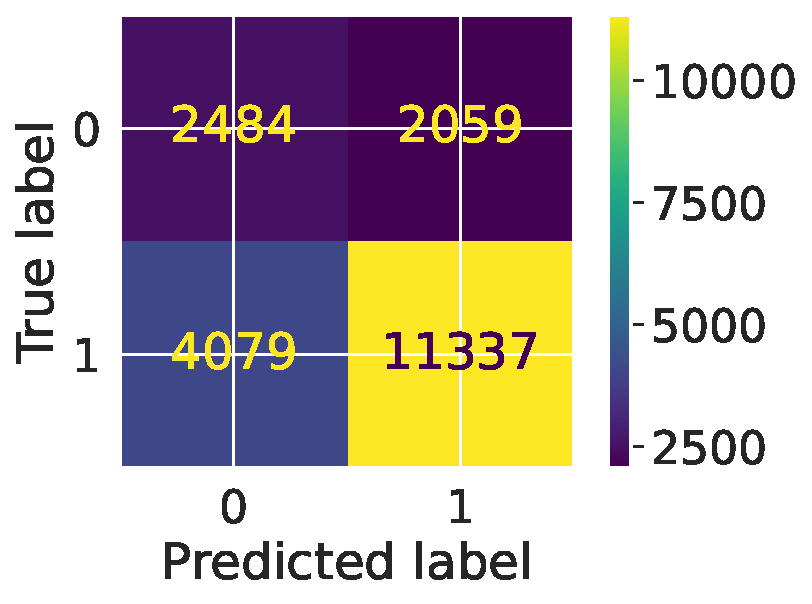
\includegraphics[width=.9\linewidth]{images/mlp_confusion_matrix_test.pdf}
      \caption{Test dataset confusion matrix for the Multilayer Perceptron}
      \label{fig:cm_mlp_test}
    \end{minipage}
\end{figure}

\subsection{Results Comparison}
We report the table of precision, recall and F-score for the rejected loans and MSE for each algorithm on the training dataset:
\begin{center}
\rowcolors{1}{gray!25}{white}     
    \begin{tabular}{l cl cl cl rl}
    \rowcolor{gray!70}
    \multicolumn{5}{c}{\textbf{Comparison of metrics on the test dataset}}\\
    \hline
    \rowcolor{gray!50}
         & \textbf{XGBoost} & \textbf{CatBoost} & \textbf{Light GBM} & \textbf{MLP}\\
         \text{Precision} & 0.7611 & \textbf{0.8916} & 0.4136 & 0.3785\\
         \text{Recall} & 0.2650 & 0.2335 & \textbf{0.6302} & 0.5468\\
         \text{F-score} & 0.3931 & 0.3701378 & \textbf{0.4994} & 0.4473 \\
         \text{MSE} & 0.1862 & 0.1809 & \textbf{0.1797} & 0.3109 \\
    \end{tabular}
\end{center}

The results show that LightGBM could achieve a lower MSE error and also beat the others for Recall and F-score on the class of Unpaid Loans. The MLP could not beat the competition, however we have to notice that the competing models are state of the art for classification on similar datasets. Classifications on others such as images would have probably achieved different results.

Even though the precision of LightGBM is lower than i.e., XGBoost and CatBoost, we can see how  LightGBM shines in a much higher Recall and F-score. In practice, the Recall becomes higher when the number of False Negatives is lower i.e., the number or loan statuses predicted as "Fully paid" incorrectly. A bank would be probably more interested in having a higher number of Recall, because the number of actual prediction for people going to default loans will be higher (see the Figures about confusion matrices).

Even though not being too "precise", it could be more important to detect more possible "bad" customers with a higher recall and perhaps being more careful about that cluster. In this respect, even the Multilayer Perceptron turned out to be better than the former two Boosting Algorithms.


\subsection{Clustering and prediction for UCI Credit Card Dataset}
In this section, we use another dataset, namely the UCI Credit Card Dataset \footnote{Source: \href{https://www.kaggle.com/uciml/default-of-credit-card-clients-dataset}{UCI}}. Information about the features are available at the link.

This dataset has as target the prediction of \textit{defaulting} probability in the next month i.e., not being able to pay, which is labeled as 1. In other words, the results are switched when comparing the inability to pay the next month, but we apply the same type of analysis.

\begin{figure}[h!]
    \centering
    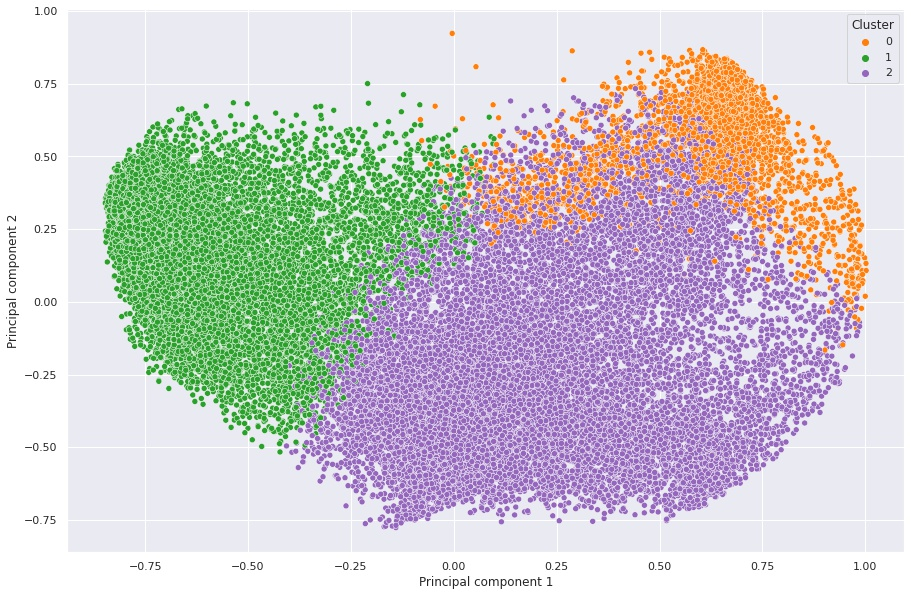
\includegraphics[width=0.9\textwidth]{images/pca_results_uci.jpg}
    \caption{PCA results on the clustering}
    \label{fig:pca_uci}
\end{figure}


\begin{center}
\rowcolors{2}{gray!25}{white}     
    \begin{tabular}{l l l l l}
    \rowcolor{gray!50}
         \textbf{Loan Status} & \textbf{Cluster 0} & \textbf{Cluster 1} & \textbf{Cluster 2}\\
         \hline
         \text{Payment} & 81.1947 & 83.5468  & 73.3544\\
         \text{Payment Default} & 18.8053 & 16.4532 & 26.6456 \\
    \end{tabular}
\end{center}

As we can see, Cluster 2 has a much higher percentage of defaulting customers when compared to others.
\begin{figure}[h!]
    \centering
    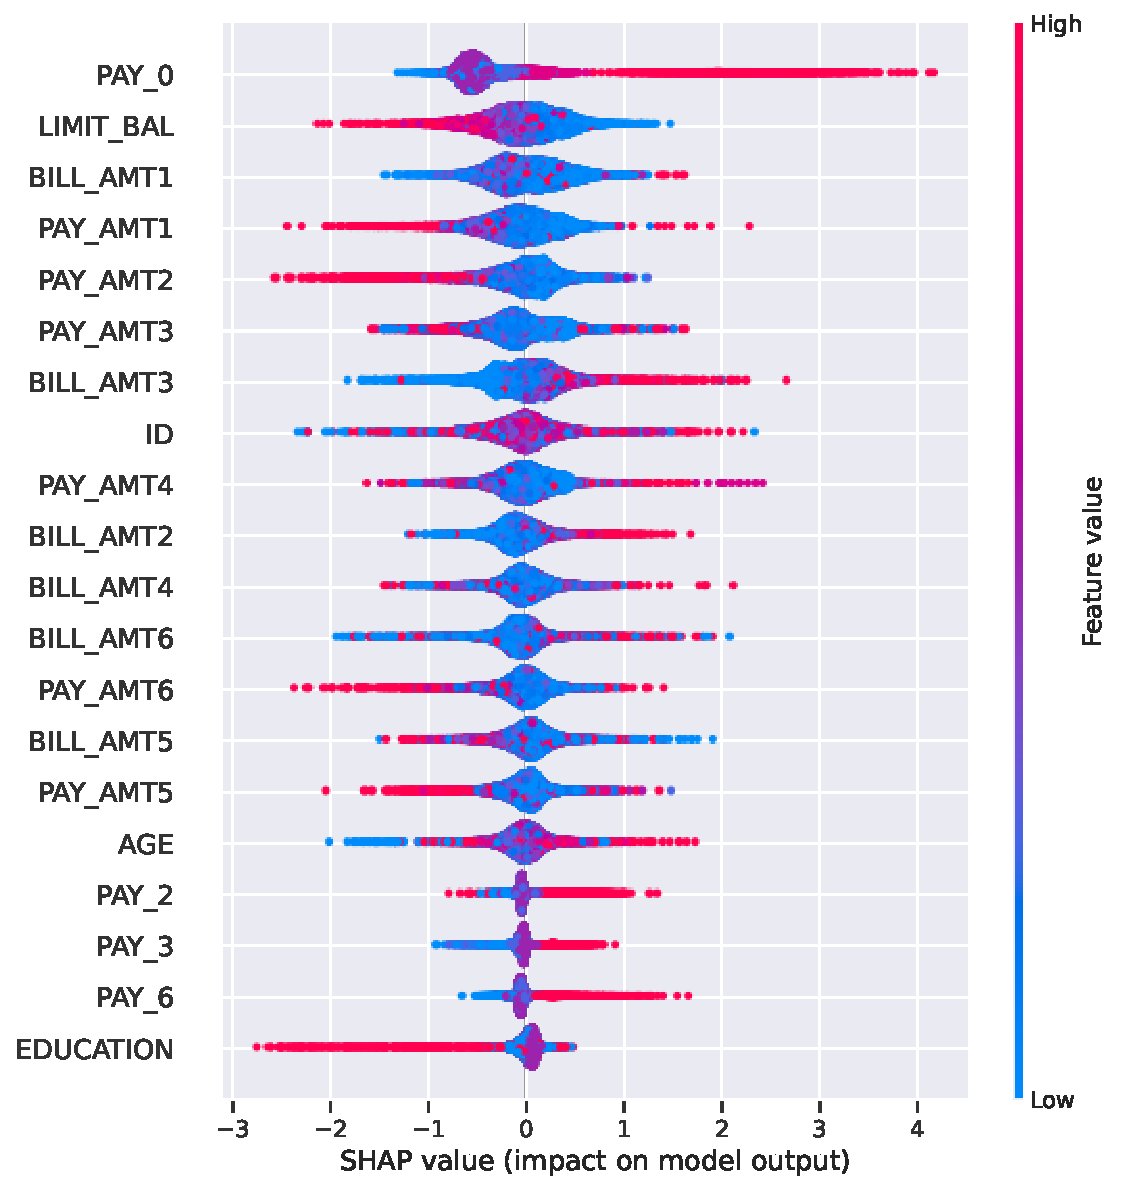
\includegraphics[width=0.9\textwidth]{images/summary_plot_uci.pdf}
    \caption{Summary SHAP plot for training data and XGBoost predictions}
    \label{fig:summary_uci}
\end{figure}

The results show that $\tt PAY\_0$ is the most important feature for determining the model's result: the feature indicates if the customer has repaid the loan in September 2005. $\tt LIMIT\_BAL$ indicates the amount of credit and $\tt BILL\_AMT1$ is the amount of bill statement. Interestingly, the credit score is the second most important feature for both datasets.

\begin{center}
\rowcolors{1}{gray!25}{white}     
    \begin{tabular}{l cl cl cl rl}
    \rowcolor{gray!70}
    \multicolumn{5}{c}{\textbf{Comparison of metrics on the test dataset}}\\
    \hline
    \rowcolor{gray!50}
         & \textbf{XGBoost} & \textbf{CatBoost} & \textbf{Light GBM} & \textbf{MLP}\\
         \text{Precision} & 0.5968 & \textbf{0.6667} & 0.4535 & 0.4085\\
         \text{Recall} & 0.3663 & 0.3625 & \textbf{0.6275} & 0.5065\\
         \text{F-score} & 0.4540 & 0.4697 & \textbf{0.5265} & 0.4522 \\
         \text{MSE} & 0.1928 & 0.1792 & \textbf{0.1742} & 0.2940 \\
    \end{tabular}
\end{center}

We consider Precision, Recall, F-score for the test data of defaulting customers and the Mean Squared Error metric. We can see how the previous results match these: Light GBM is able to obtain better results with Recall, F-score and the MSE metrics.


 %%%%%%%%%% BIBLIOGRAPHY %%%%%%%%%% 
\bibliographystyle{plain}
\bibliography{ref}

\end{document}